\documentclass{beamer}
\usepackage{presentation}


\begin{document}

\title{Midterm 1 Aftermath}  
% \subtitle{}
\author{Jose Abel Castellanos Joo}
\date{\today} 

\frame{\titlepage} 

% \begin{frame}[allowframebreaks]{Table of Contents}
%   \tableofcontents[sections={1-2}]
%   \framebreak
%   \tableofcontents[sections={3-5}]
% \end{frame}

% \section{Preliminaries}
\begin{frame}{Preliminaries}
Here is the text for the preliminaries slide.
\end{frame}

%%% Local Variables:
%%% mode: latex
%%% TeX-master: "main"
%%% End:

% \section{Conclusions}
\begin{frame}{Conclusions}
Here is the text for the conclusions slide.
\end{frame}

%%% Local Variables:
%%% mode: latex
%%% TeX-master: "main"
%%% End:


\section{Review}

\begin{frame}[fragile]{Let's do lets}
  \begin{figure}[htpb]
    \centering
    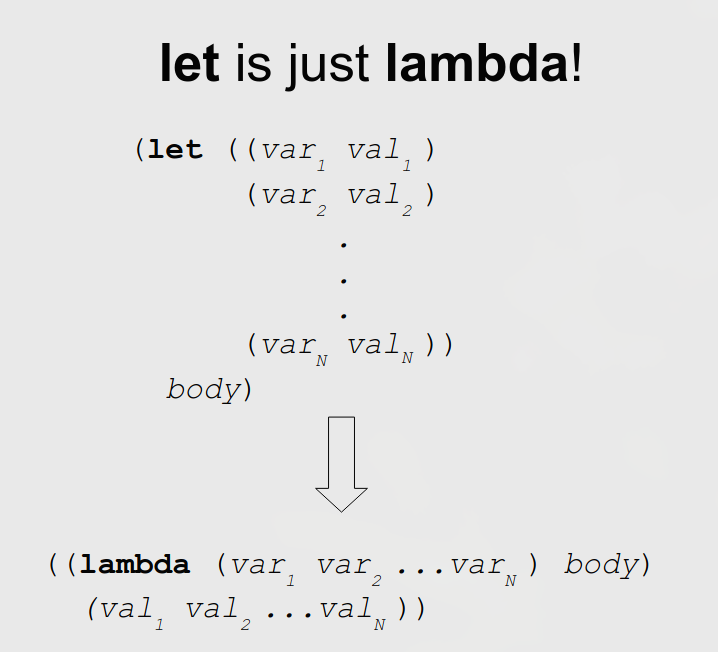
\includegraphics[width=0.6\textwidth]{./figures/let.png}
    \caption{\verb|let| s are just lambdas}
    \label{fig:let.png}
  \end{figure}

\end{frame}

\begin{frame}[fragile]{Let's do lets}
  \begin{figure}[htpb]
    \centering
    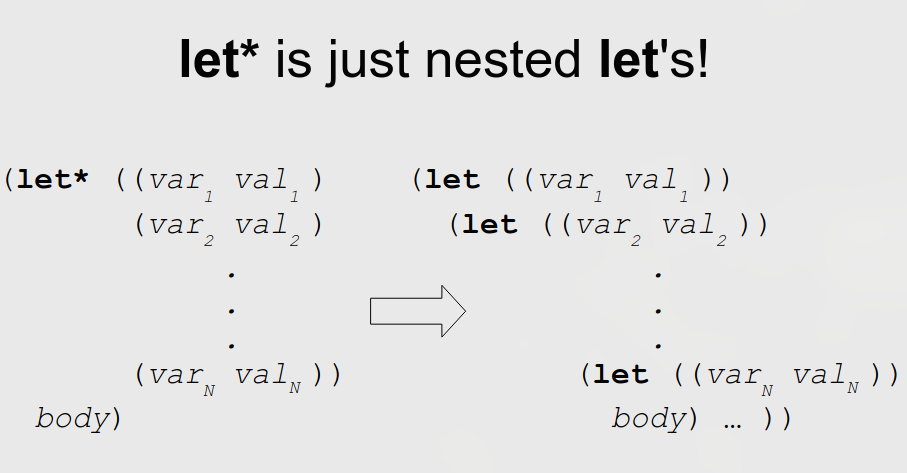
\includegraphics[width=0.8\textwidth]{./figures/let_star.png}
    \label{fig:let_star.png}
    \caption{\verb|let*| s are just \verb|let| s}
  \end{figure}
\end{frame}

\begin{frame}{Tail Positions}

  \begin{itemize}
  \item Tail positions are shown in red:
    \begin{itemize}
    \item (\textbf{if} pred {\color{red} $val_1$} {\color{red} $val_2$})
    \item (\textbf{cond} ($pred_1$ {\color{red} $val_1$}) $\dots$
      ($pred_{N-1}$ {\color{red} $val_{N-1}$})
      (else {\color{red} $val_N$}))
    \item (\textbf{ord} $pred_1$ $pred_2$ $\dots$ $pred_{N-1}$ {\color{red} $pred_N$} )
    \item (\textbf{and} $pred_1$ $pred_2$ $\dots$ $pred_{N-1}$ {\color{red} $pred_N$} )
    \end{itemize}
  \item These positions within special forms in tail positions are also tail positions!

    e.g:

    \begin{itemize}
    \item (\textbf{if} pred {\color{red} $val_1$} (\textbf{if} pred {\color{red} $val_2$} {\color{red} $val_3$}))
    \item (\textbf{cond} ($pred_1$ {\color{red} $val_1$}) $\dots$
      ($pred_{N-1}$ (\textbf{if} pred {\color{red} $val_1^{'}$} {\color{red} $val_2^{'}$}))
      (else (\textbf{and} $pred_1^{'}$ $pred_2^{'}$ $\dots$ $pred_{N-1}^{'}$ {\color{red} $pred_N$} )))
    \end{itemize}

  \end{itemize}
\end{frame}

\begin{frame}[fragile]{Tail positions in special forms}
  \begin{figure}[htpb]
    \centering
    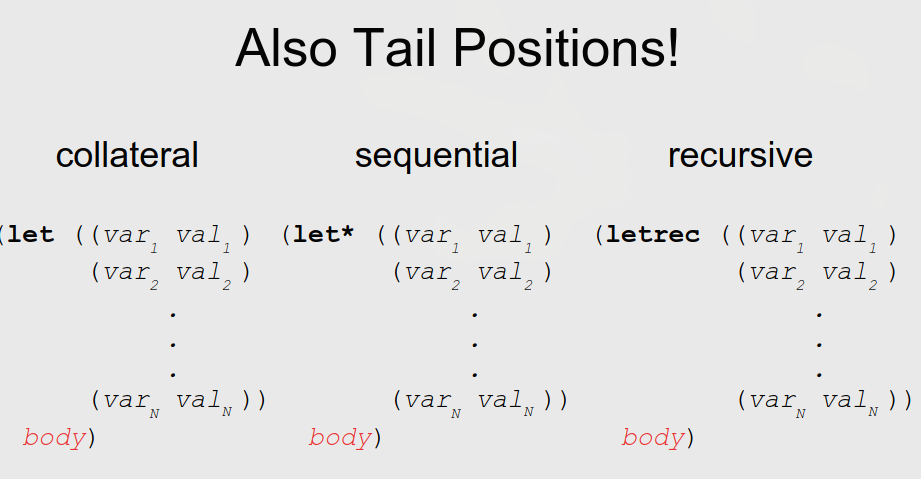
\includegraphics[width=0.8\textwidth]{./figures/special_forms_tail_positions.png} 
    \caption{Tail positions in some special forms}
    \label{fig:special_forms_tail_positions}
  \end{figure}
  
\end{frame}

\begin{frame}[fragile]{Top position}
  \begin{itemize}
  \item If $a$ is a constant, $a$ is the top position
  \item If \verb|(f arg1 arg2 ... argn)| is a function application, $f$ is the
    top position
  \end{itemize}
\end{frame}

\begin{frame}[fragile]{Tail recursive functions}
  Recursive functions such that the recursive call only happens at the tail
  positions in the top position
\end{frame}

\begin{frame}[fragile]{Thinking all possible cases}
  Review last exercise of midterm I
\end{frame}

% \begin{frame}[allowframebreaks]
%   \frametitle{References}
%   %   \bibliographystyle{plain}
%   %   \bibliography{references}
% \end{frame}

\end{document}

